%Document-Author: Davide Tommasin
%Document-Date: 2016/05/12
%Document-Description: Manuale Utente del gruppo SWEeneyThreads 

\documentclass[a4paper]{article}
\usepackage[english, italian]{babel}
\usepackage[T1]{fontenc}
\usepackage[utf8]{inputenc}
\usepackage{url}
\usepackage{graphicx}
\usepackage[hidelinks]{hyperref}
\usepackage{booktabs}
\usepackage{eurosym}
\usepackage{tabularx}
\usepackage{pifont}
\usepackage[table]{xcolor}
\usepackage{float}
\usepackage[]{appendix}
\usepackage{ltxtable} 
\usepackage{geometry}
\geometry{margin=1in}
\usepackage{longtable}
\usepackage{multirow}

\graphicspath{{Immagini/}}

\newcolumntype{Y}{>{\centering\arraybackslash}X}
\newcolumntype{s}{>{\hsize=.21\hsize}X}
\newcolumntype{f}{>{\hsize=.37\hsize}X}
\newcolumntype{m}{>{\hsize=.42\hsize}X}
\newcolumntype{t}{>{\hsize=.1\hsize}X}
\newcolumntype{r}{>{\hsize=.3\hsize}X}
\newcolumntype{k}{>{\hsize=.4\hsize}X}

\renewcommand{\abstractname}{Tabella contenuti}

\begin{document}
	
	\begin{titlepage}
		% Defines a new command for the horizontal lines, change thickness here
		\newcommand{\HRule}{\rule{\linewidth}{0.5mm}} 
		\center  
		
		% HEADING SECTION
		\textsc{\LARGE SWEeneyThreads}\\[1.5cm] 
		\textsc{\Large Actorbase}\\[0.5cm] 
		\textsc{\large a NoSQL DB based on the Actor model}\\[0.5cm]
		
		
		% TITLE SECTION
		\HRule \\[0.4cm]
		{ \huge \bfseries User Manual}\\[0.4cm] 
		\HRule \\[1.5cm]
		
		% AUTHOR SECTION
		\begin{minipage}{0.4\textwidth}
			\begin{flushleft} \large
				\emph{Redattori:}\\
				Maino Elia \newline
				Tommasin Davide \\
			\end{flushleft}
		\end{minipage}
		~
		\begin{minipage}{0.4\textwidth}
			\begin{flushright} \large
				\emph{Approvazione:} \\
				\emph{Verifica:} 
			\end{flushright}
		\end{minipage}
		
		%immagine
		\begin{figure}[H]
			\centering
			
\includegraphics[scale=0.8]{sweeney.png}
		\end{figure}
		\begin{center}
			Versione 1.0.2
		\end{center}
		% Date, change the \today to a set date if you want to be precise
		{\large \today}\\[3cm] 
		% Fill the rest of the page with whitespace
		\vfill  
	\end{titlepage}
	
	
	\tableofcontents
	
	\newpage
	\section*{History log}
		\LTXtable{\textwidth}{Tabelle/tabelle_diario_modifiche/tabella_manualeutenteENG.tex}	

	\newpage 
    \section{Introduction}
	\subsection{Document's purpose}
		The present document represents the user manual for the use of \emph{Actorbase}, a No-SQL database. All the user application's features will be described in detail. The manual i dividend into three main sections, related to the main components of the product: Client, Server and Driver.
	\subsection{Product's purpose}
		The project's purpose is the development of a key-value NoSQL Database based on the actor model, with the goal of supply an appropriate technology for the development of modern applications which request very short response time, and which elaborate huges quantities of data. The development will lead to the release of the software under MIT license.
	\subsection{Glossary}
		In order to avoid language ambiguities, and to maximize documents' comprehension, the group wrote \emph{Glossario v2.0.0}. In it will be defined, in a clear and concise way, the terms which could lead to ambiguities or text incomprehensions.
	\subsection{References}
	\subsubsection{Normative}
		\begin{itemize}
			\item \textbf{Norme di progetto:} \emph{Norme di progetto v3.0.0}
			\item \textbf{Capitolato d'appalto Actorbase (C1):} \\ 
			\url{http://www.math.unipd.it/~tullio/IS-1/2015/Progetto/C1p.pdf}
		\end{itemize}
	\newpage

	\section{Actorbase}
	\emph{Actorbase} is a key-value No-SQL database based on the actor model, which guarantees high level of scalability, resilience and performance. It allows to manage easily and flexibly your data, using the mein advantages offered by the actor model, in order to support the development of modern and performing applications.
	\\ \\
	\emph{Actorbase} provides a command line client interface which offers an easy way to handle data as strings, with it it is possible to communicate quickly and intuitively with a server.
	\\ \\
	For more flexible queries it's avaiable the \emph{Scala} driver, integrable with every application.
	\begin{figure}[H]
		\centering
		
\includegraphics[scale=0.4]{actorbaseLogo.png}
		\caption{Actorbase Logo}
	\end{figure}

	\newpage



	\section{System requirements}	
	The correct execution of \emph{Actorbase} is guarantedd on machines that meet the subsequent hardware and software specifications.
	\\ \\
	OS:
	\begin{itemize}
		\item Windows 7 or newer
		\item OS X 10.7 or newer
		\item Ubuntu 14.04 or newer
	\end{itemize}
	Java Virtual Machine (JVM) 8 or newer.
	\\ \\
	RAM:
	\begin{itemize}
		\item Client application: 2GB minimum
		\item Server application: 4GB minimum, 8GB recommended
	\end{itemize}
	There aren't explicit requirements for the processor architecture or speed. Using a very old processor could slow down the system usage.

	\section{Installation}
	\emph{Actorbase} runs on JVM, that's the reason why it doesn't need an installation procedure (just click on the launch icon). 
	\newpage



	\section{Server application}
	The server application allows to run and manage an \emph{Actorbase} server instance on the machine. Once startes, the server allows clients to connect to the machine, and to query the database.
	
	\subsection{Server configuration}
	The server machine's configuration is made changing \texttt{server.conf} file. The configuration file allows the administrator to set the IP address and the connection port.
	\\
	If the user tries to run the server application without have defined the configuration parameters, the server will display an error message and won't start.
	
	\subsection{Server interface}
	Once the administrator has modified the configuration file it is possible to start the application by click on the icon. The server application provides the user a command line interface which displays the operation log in real time.
	\begin{figure}[H]
		\centering
		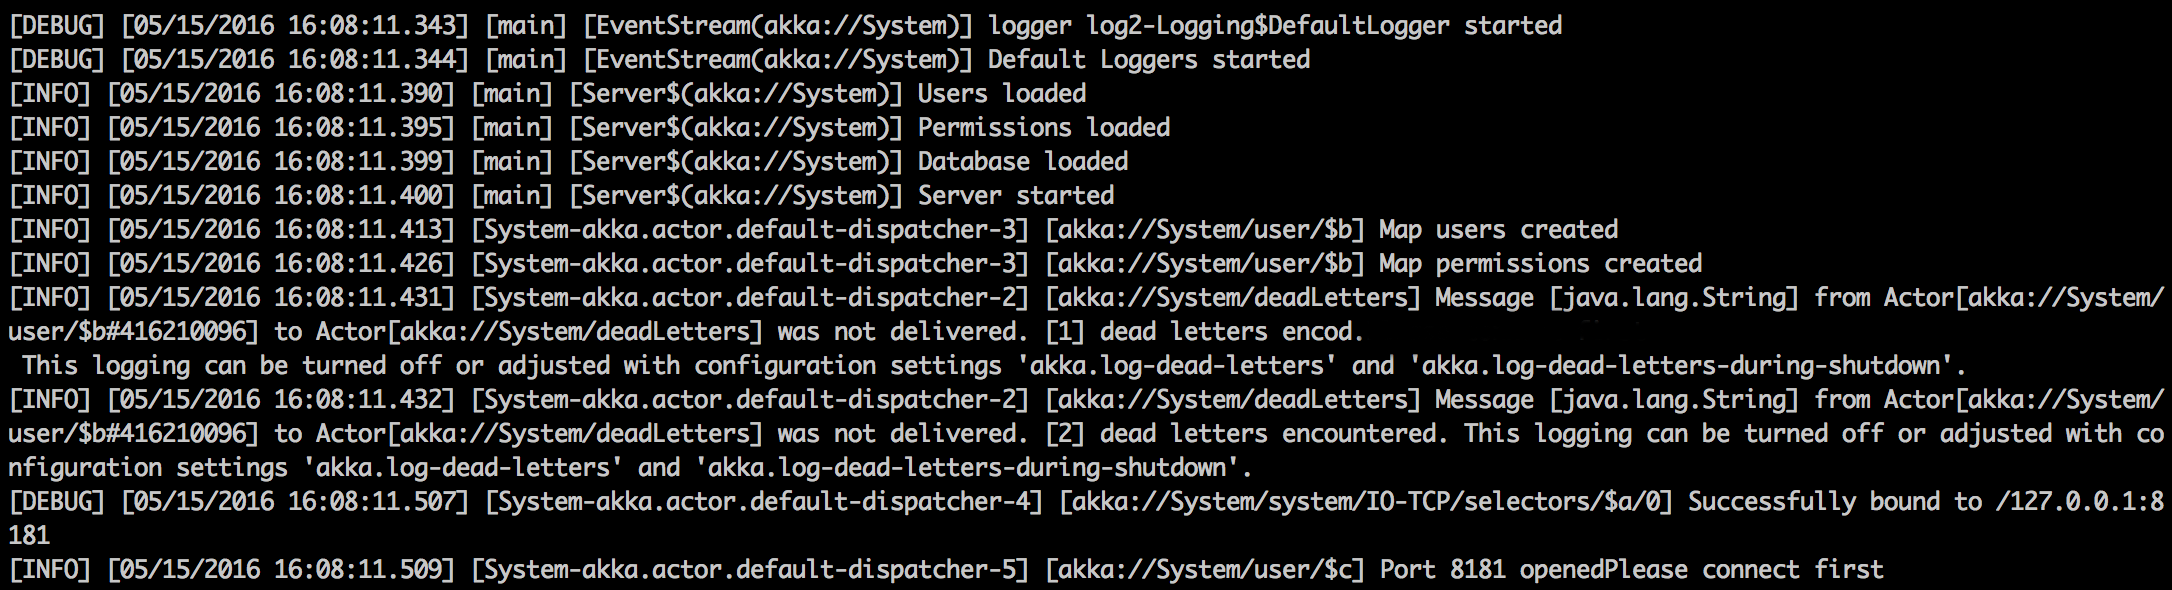
\includegraphics[width=\textwidth]{logServer.png}
		\caption{Server's log interface}
	\end{figure}
	\newpage
	

	\section{Client application}
	The client application provides the user a command line interface to connect to an \emph{Actorbase} server, and to query the database. To start the client, just double-click on the client's icon. Once strarted the clients presents the user a welcome banner, followed by a brief description of thr software configuration used (JVM version and operating system).
	\begin{figure}[H]
		\centering
		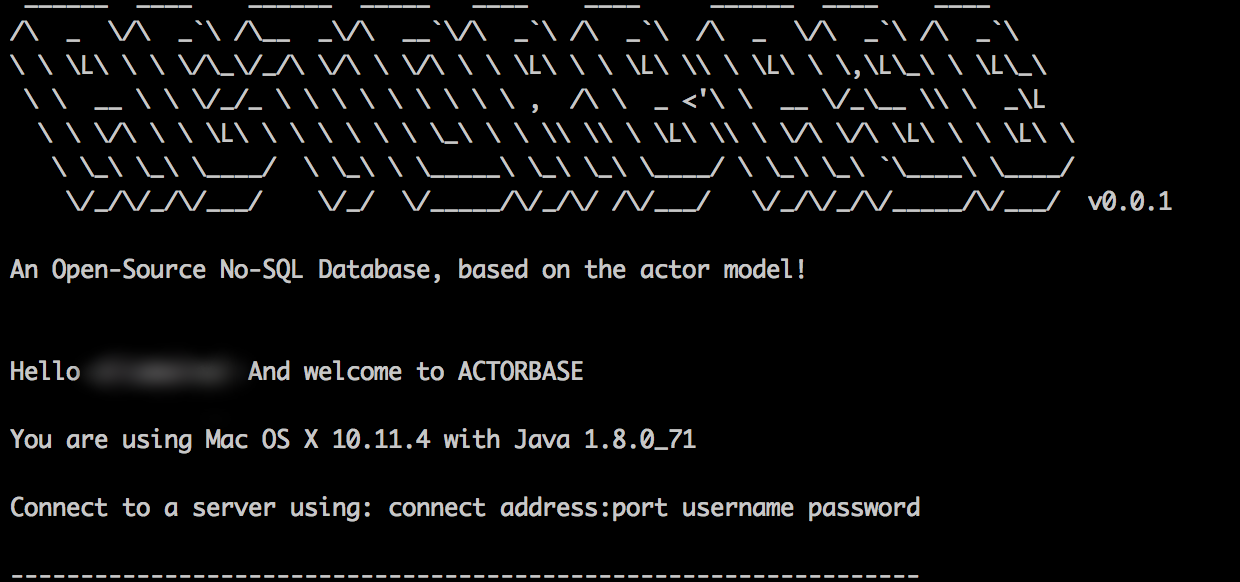
\includegraphics[width=\textwidth]{welcomeClient.png}
		\caption{Client's welcome banner}
	\end{figure}
	The interaction with the client interface is made with textual commands, they can be composed of multiple fields, separated by a space character.
	
	\subsection{Connection management}
	Once started the client, the first thing to do is connect to a server, the connection management is based on two commands: \texttt{connect} and \texttt{disconnect}. The application doesn't allow to manage more than one connection at time.
	
	\subsubsection{\texttt{connect} command}
	This command allows the user to connect to a server, the command structure is:
	\\ \\
	\texttt{actorbase>	connect address username password}
	\\ \\
	The server addres has to be written in the format \texttt{serverAddress:port}. \\ \\
	In case of success, the user receives a confirm message (\texttt{"You are connected!"}), if not the user receives an error message (\texttt{"Connection failed!"}).
	
	\subsubsection{\texttt{disconnect} command}
	To disconnect from the server, the user just has to insert the command \texttt{disconnect} and press entry.
	

	\subsection{Inline help}
	It is possible to obtain an help for the allowed operations, directly from the command line. The command \texttt{help} allows to obtain a generic help or a specific one.
	
	\subsubsection{Generic \texttt{help} command}
	Generic help command doesn't requests more parameters and prints on screen the \emph{Actorbase} commands list. Each command is followed by a brief description which explains his behaviour.
	
	\subsubsection{Specific \texttt{help} command}
	Specific help command has this structure:
	\\ \\
	\texttt{actorbase>	help commandName}
	\\ \\
	It allows to request informations for a particulare command, and to obtain a description of it.
	
	\subsection{Server level operations commands}
	Once connected the user is at "server level". At that level the user can do operation on the databases like:
	\begin{itemize}
		\item Show the databases list
		\item Select a database
		\item Create a database
		\item Remove a database
	\end{itemize}
	
	\subsubsection{\texttt{listdb} command}
	This command allows the user to obtain, printed on screen, the list of databases of which the user has some access permission. The command does not request additional parameters.
	\\ \\
	\texttt{actorbase>	listdb}

	\subsubsection{\texttt{selectdb} command}
	This command allows the user to select a database. Once selected a database, the user can execute operation on the maps of it. The command structure is the sequent:
	\\ \\
	\texttt{actorbase>	selectdb databaseName}
	\\ \\
	In case the user has the requested permissions, he receives a confirmation message: \texttt{"Database x selected"}. If not an invalid operation is reported.

	\subsubsection{\texttt{createdb} command}
	This commands allows the user to create a new database with the name specified, in case a database with that name isn't present already.
	\\ \\
	\texttt{actorbase>	createdb databaseName}
	\\ \\
	If a database with the inserted name already exists the creation fails, the user receives an error message: \texttt{"A database with the requested name already exists"}.

	\subsubsection{\texttt{deletedb} command}
	This command allows the user to delete a database from the server:
	\\ \\
	\texttt{actorbase>	deletedb databaseName}
	\\ \\
	If the user tries to 
	Nel caso si tenti di rimuovere un database inesistente o di cui non si dispone dei permessi di modifica, l'utente riceve un messaggio di operazione non valida (\texttt{"Invalid operation"}).
	

	\subsection{Comandi per operazioni a livello database}
	Una volta selezionato un database tramite il comando \texttt{selectdb}, l'utente si trova a "livello database". A tale livello si possono effettuare queste operazioni:
	\begin{itemize}
		\item Visualizzazione della lista delle mappe che compongono il database
		\item Selezione di una mappa
		\item Creazione di una mappa
		\item Eliminazione di una mappa
	\end{itemize}

	\subsubsection{\texttt{listmap} command}
	Questo comando stampa una lista di tutte le mappe che compongono il database precedentemente selezionato.
	\\ \\
	\texttt{actorbase>	listmap}

	\subsubsection{\texttt{selectmap} command}
	Questo comando permette di selezionare una mappa, utilizzando la seguente sintassi:
	\\ \\
	\texttt{actorbase>	selectmap nomeMappa}
	\\ \\
	La selezione viene confermata in caso di successo con il messaggio \texttt{"Map x selected"}, altrimenti si riceve un messaggio di operazione non valida (\texttt{"Invalid operation"}).

	\subsubsection{\texttt{createmap} command}
	Questo comando permette di creare una mappa con il nome inserito, all'interno del database selezionato.
	\\ \\
	\texttt{actorbase>	createmap nomeMappa}
	\\ \\
	La creazione viene confermata in caso di successo con il messaggio \texttt{"Map x created"}. Nel caso non si disponga dei permessi di modifica al database, o esista già una mappa con il nome inserito, si riceve un messaggio di operazione non valida (\texttt{"Invalid operation"}).

	\subsubsection{\texttt{deletemap} command}
	Questo comando permette di eliminare una mappa dal database selezionato. 
	\\ \\
	\texttt{actorbase>	deletemap nomeMappa}
	\\ \\
	L'eliminazione viene confermata in caso di successo con il messaggio \texttt{"Map x removed"}. Nel caso non si disponga dei permessi di modifica al database, o la mappa richiesta non esista, si riceve un messaggio di operazione non valida (\texttt{"Invalid operation"}).
	

	\subsection{Comandi per operazioni a livello mappa}
	Una volta selezionata una mappa tramite il comando \texttt{selectmap}, l'utente si trova a "livello mappa". A tale livello si possono effettuare queste operazioni:
	\begin{itemize}
		\item Visualizzazione della lista delle chiavi
		\item Ricerca di un item per chiave
		\item Inserimento di un item 
		\item Aggiornamento di un item
		\item Rimozione di un item
	\end{itemize}

	\subsubsection{\texttt{keys} command}
	Questo comando permette di visualizzare la lista di tutte le chiavi degli item che compongono la mappa selezionata.
	\\ \\
	\texttt{actorbase>	keys}

	\subsubsection{\texttt{find} command}
	Questo comando permette di ottenere il valore di un item della mappa, effettuando la ricerca tramite la sua chiave.
	\\ \\
	\texttt{actorbase>	find key}
	\\ \\
	Nel caso sia presente un item corrispondente alla chiave inserita, si riceve il valore dell'item in formato stringa, stampato a video. Se l'item non viene trovato si riceve un messaggio di errore.
	\subsubsection{\texttt{remove} command}
	Questo comando permette di rimuovere un item dalla mappa, ricercandolo tramite la chiave.
	\\ \\
	\texttt{actorbase>	remove key}
	\\ \\
	L'eliminazione viene confermata in caso di successo con il messaggio \texttt{"Item removed"}. Nel caso non si disponga dei permessi di modifica al database, o l'item 
	richiesto non esista, si riceve un messaggio di operazione non valida (\texttt{"Invalid operation"}).

	\subsubsection{\texttt{insert} command}
	Questo comando permette di inserire un item (coppia chiave-valore) nella mappa:
	\\ \\
	\texttt{actorbase>	insert key value}
	\\ \\
	L'inserimento viene confermato in caso di successo con il messaggio \texttt{"Item inserted"}. Nel caso non si disponga dei permessi di modifica al database, o sia già presente un item con la chiave inserita, si riceve un messaggio di operazione non valida (\texttt{"Invalid operation"}).
	
	\subsubsection{\texttt{update} command}
	Questo comando permette di aggiornare un item dalla mappa, ricercandolo tramite la chiave e inserendo il valore aggiornato.
	\\ \\
	\texttt{actorbase>	update key value}
	\\ \\
	L'aggiornamento viene confermato in caso di successo con il messaggio \texttt{"Item updated"}. Nel caso non si disponga dei permessi di modifica al database, o l'item 
	richiesto non esista, si riceve un messaggio di operazione non valida (\texttt{"Invalid operation"}).
			
	\cleardoublepage
	\addcontentsline{toc}{section}{\listfigurename}
	\listoffigures
	
	\cleardoublepage
	\addcontentsline{toc}{section}{\listtablename}
	\listoftables
		
\end{document}